\let\negmedspace\undefined
\let\negthickspace\undefined
\documentclass[journal]{IEEEtran}
\usepackage[a5paper, margin=10mm, onecolumn]{geometry}
%\usepackage{lmodern} % Ensure lmodern is loaded for pdflatex
\usepackage{tfrupee} % Include tfrupee package

\setlength{\headheight}{1cm} % Set the height of the header box
\setlength{\headsep}{0mm}     % Set the distance between the header box and the top of the text

\usepackage{gvv-book}
\usepackage{gvv}
\usepackage{cite}
\usepackage{amsmath,amssymb,amsfonts,amsthm}
\usepackage{algorithmic}
\usepackage{graphicx}
\usepackage{textcomp}
\usepackage{xcolor}
\usepackage{txfonts}
\usepackage{listings}
\usepackage{enumitem}
\usepackage{mathtools}
\usepackage{gensymb}
\usepackage{comment}
\usepackage[breaklinks=true]{hyperref}
\usepackage{tkz-euclide} 
\usepackage{listings}
% \usepackage{gvv}                                        
\def\inputGnumericTable{}                                 
\usepackage[latin1]{inputenc}                                
\usepackage{color}                                            
\usepackage{array}                                            
\usepackage{longtable}                                       
\usepackage{calc}                                             
\usepackage{multirow}                                         
\usepackage{hhline}                                           
\usepackage{ifthen}                                           
\usepackage{lscape}
\begin{document}

\bibliographystyle{IEEEtran}
\vspace{3cm}

\title{1.4.9k}
\author{AI24BTECH11031 - Shivram S
}
% \maketitle
% \newpage
% \bigskip
{\let\newpage\relax\maketitle}

\renewcommand{\thefigure}{\theenumi}
\renewcommand{\thetable}{\theenumi}
\setlength{\intextsep}{10pt} % Space between text and floats


\numberwithin{equation}{enumi}
\numberwithin{figure}{enumi}
\renewcommand{\thetable}{\theenumi}


\textbf{Question: }\\
Find the position vector of a point $\vec R$ which divides the line joining two points $\vec P$ and $\vec Q$ whose position vectors are $\hat{i} + 2 \hat{j} - \hat{k}$ and $-\hat{i} + \hat{j} + \hat{k}$ respectively, in the ratio $2:1$

\begin{enumerate}
	\item internally
	\item externally
\end{enumerate}

\textbf{Solution: } \\
\begin{enumerate}
	\item Using section formula (1.1.4.1), the desired point is 
		\begin{align}
			\vec{R} = \frac{\vec{Q} + \frac{1}{2}\vec{P}}{1 + \frac{1}{2}} = \frac{1}{1 + \frac{1}{2}}\brak{\myvec{-1 \\ 1 \\ 1} + \frac{1}{2}\myvec{1 \\ 2 \\ -1}} = \myvec{-\frac{1}{3} \\ \frac{4}{3} \\ \frac{1}{3}}	
		\end{align}
		\begin{figure}[h!]
			\centering
			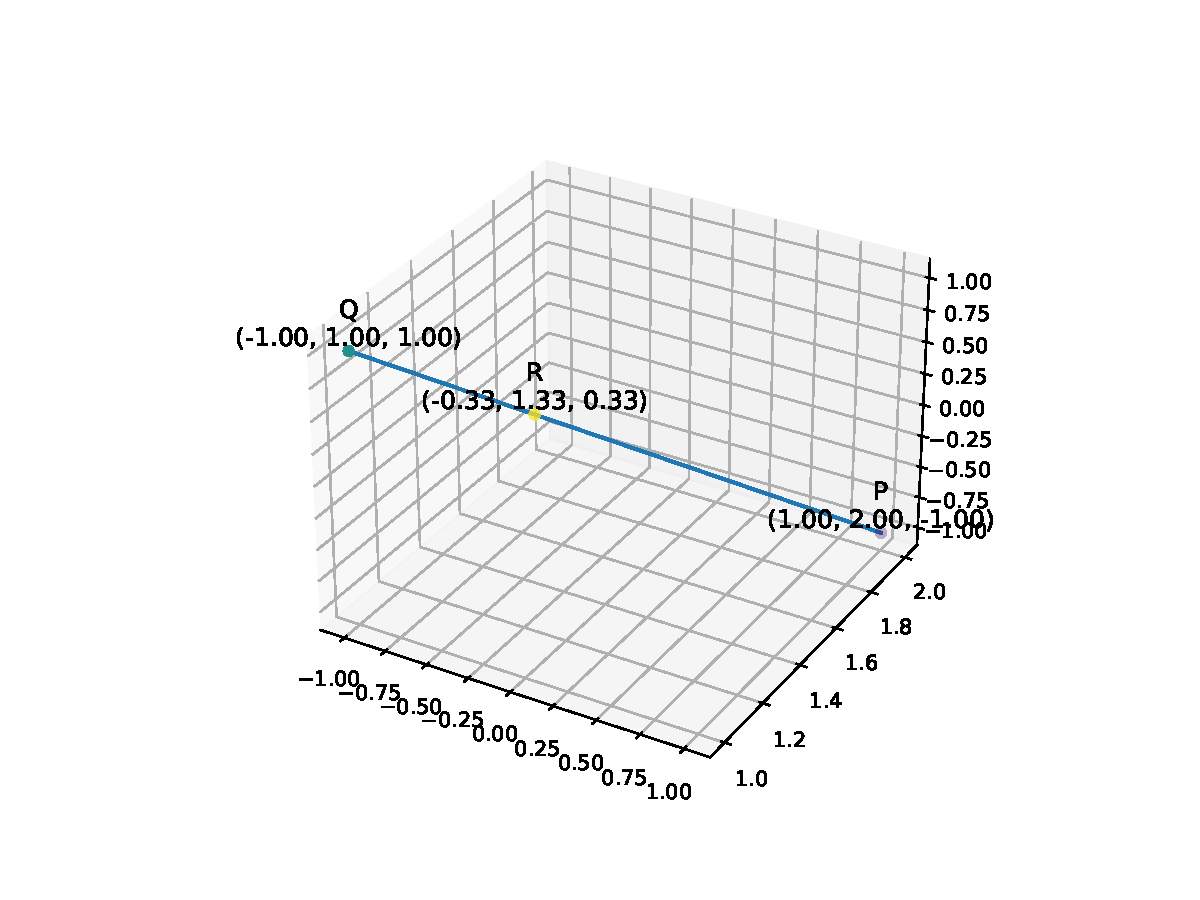
\includegraphics[width=0.7\linewidth]{figs/fig1.pdf}
			\caption{R divides PQ internally in the ratio 2:1}
		\end{figure}
	\item Using section formula (1.1.4.1), the desired point is 
		\begin{align}
			\vec{R} = \frac{\vec{Q} - \frac{1}{2}\vec{P}}{1 - \frac{1}{2}} = \frac {1}{1 - \frac{1}{2}} \brak{\myvec{-1 \\ 1 \\ 1} - \frac{1}{2}\myvec{1 \\ 2 \\ -1}} = \myvec{-3 \\ 0 \\ 3}
		\end{align}
		\begin{figure}[h!]
			\centering
			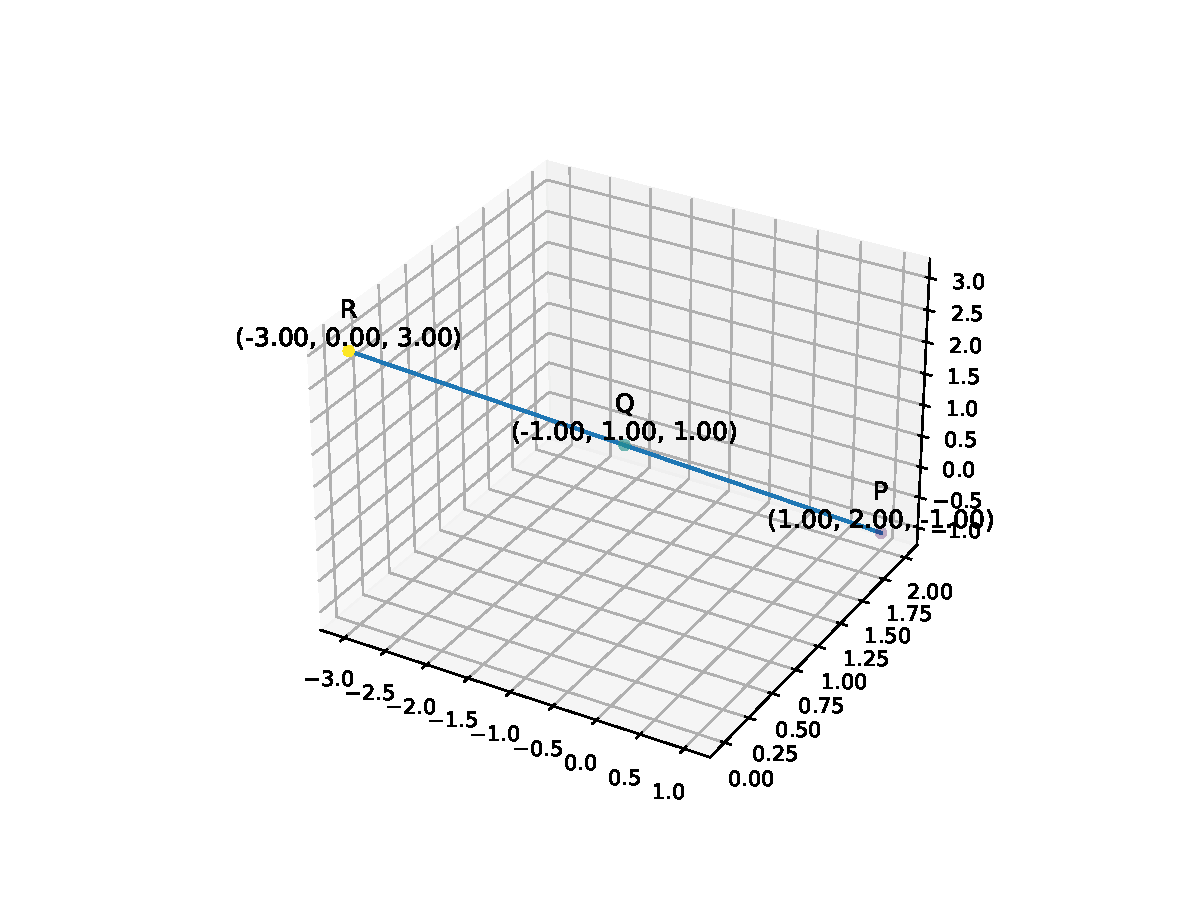
\includegraphics[width=0.7\linewidth]{figs/fig2.pdf}
			\caption{R divides PQ externally in the ratio 2:1}
		\end{figure}
\end{enumerate}
\end{document}



